\documentclass{report}

% Package necessari
\usepackage[a4paper]{geometry}
\usepackage[utf8]{inputenc}
\usepackage[italian]{babel}
\usepackage[T1]{fontenc}
\usepackage{amsmath}
\usepackage{amssymb}
\usepackage{graphicx}
\usepackage[table, dvipsnames]{xcolor}
\usepackage{listings}
\usepackage{hyperref}
\usepackage{enumitem}
\usepackage{fancyhdr}
\usepackage{algorithm}
\usepackage[noend]{algpseudocode}
\usepackage[font={small,sl}]{caption}
\usepackage[font={small,sl}]{subcaption}

% Impostazione delle lunghezze di alcuni elementi del documento
\setlength{\parskip}{1em}
\setlength{\parindent}{0em}
\setlength{\arrayrulewidth}{0.1em}

% Informazioni per la title page
\title{\small{Corso di Performance Modeling of Computer Systems \& Networks} \\
\huge{Studio delle prestazioni di un Ufficio Postale di \\
\textbf{Poste Italiane}}}

\date{A.A. 2020/2021}

\author{A. Chillotti\thanks{\texttt{\href{mailto:alessandro.chillotti@outlook.it}{alessandro.chillotti@outlook.it}}}
\and 
C. Cuffaro\thanks{\texttt{\href{mailto:cristiano.cuffaro@outlook.com}{cristiano.cuffaro@outlook.com}}} 
\and 
S. Tiberi\thanks{\texttt{\href{mailto:simone.tiberi.98@gmail.com}{simone.tiberi.98@gmail.com}}}
}

% Impostazione del package hyperref
\hypersetup{
    colorlinks=true,
    linktocpage=true,
    linkcolor=blue,
    urlcolor=blue,
    pdftitle={Studio delle prestazioni di un Ufficio Postale di Poste Italiane},
    pdfauthor={A. Chillotti, C. Cuffaro e S. Tiberi},
}

% Colori per i listing
\definecolor{code_red}{rgb}{0.6,0,0} % strings
\definecolor{code_green}{rgb}{0.25,0.5,0.35} % comments
\definecolor{code_purple}{rgb}{0.5,0,0.35} % keywords
\definecolor{code_background}{rgb}{0.95,0.95,0.92} % background

% Altri colori
\definecolor{forestgreen}{rgb}{0.13, 0.55, 0.13}
\definecolor{airforceblue}{rgb}{0.36, 0.54, 0.66}
 
% Stile del codice standard (C)
\lstset{
	language=C, 
	backgroundcolor=\color{code_background},
	frame=single,
	basicstyle=\ttfamily\small,
	keywordstyle=\color{code_purple}\bfseries\small,
	stringstyle=\color{code_red}\small,
	commentstyle=\color{code_green}\small,
	numbers=left,
	numberstyle=\small\color{gray},
	numbersep=5pt,
	tabsize=4,
	showtabs=false,
	showspaces=false,
	showstringspaces=false,
	escapechar=|, 
	captionpos=b,
	breaklines=true,
}

\pagestyle{fancy}
\fancyhf{}
\lhead{\small A.Chillotti, C. Cuffaro, S. Tiberi}
\rhead{\small Performance Modeling of Computer Systems \& Networks}
\cfoot{\thepage}
%\cfoot{Pagina \thepage}

% Spaziatura tabelle
\renewcommand{\arraystretch}{1.5}

\graphicspath{ {./figs/} }
% Definizione del colore delle tabelle
\newcommand{\tablecolors}[1][2]{\rowcolors{#1}{yellow!50}{yellow!25}}

% Definizione dello stile da usare per la P di probabilità (grassetto in math-mode)
\newcommand{\pr}{\mathbf{P}}

% Forzatura del displaystyle in math-mode
\everymath\expandafter{\the\everymath\displaystyle}

%\newcommand{\scaption}[1]{\small{\caption{#1}}}
\newcommand{\ded}{{\color{red}\hat{k}}}

\newcommand{\uo}{\textsl{Unica Operazione}}
\newcommand{\pp}{\textsl{Pagamenti \& Prelievi}}
\newcommand{\sr}{\textsl{Spedizioni \& Ritiri}}

\renewcommand{\lstlistingname}{Snippet}

\begin{document}
\maketitle
\tableofcontents

\chapter{Presentazione del caso di studio}\label{chp:presentazione}
Il sistema oggetto dell'analisi in questione eroga le seguenti tipologie di servizi:
\begin{enumerate}
\item \uo{} (e.g. ricarica \textsl{PostePay}, invio raccomandata e pagamento di massimo tre bollettini)
\item \pp{} (e.g. pagamento di un numero arbitrario di bollettini, bollo auto e libretti)  
\item \sr{} (e.g. invio corrispondenza, lettere, pacchi e raccomandate)
\end{enumerate}

Per essere serviti i clienti possono recarsi all'ufficio postale, prendere un ticket relativo al servizio a cui sono interessati e mettersi in coda in attesa del proprio turno. Nel caso in cui essi dimostrino di essere titolari di un conto \textsl{BancoPosta} potranno accodarsi in una fila dedicata.

Un insieme di sportelli serve le richieste degli utenti in accordo alle seguenti regole: 
\begin{enumerate}[label=R\arabic*), align=left, leftmargin=*]
\item I ticket di tipo \sr{} vengono serviti da uno sportello dedicato il quale, in assenza di questa tipologia, opera come gli altri. Il comportamento di tale servente è schematizzato in figura \ref{fig:presentazione-1}. 
\item Poiché, per definizione, ticket di tipo \uo{} dovrebbero richiedere meno tempo per essere processati, viene assegnata loro una priorità maggiore di \pp{}.
\item I clienti titolari di un conto \textsl{BancoPosta} vengono serviti con una priorità maggiore rispetto agli altri, in accordo alle regole R1 ed R2.
\end{enumerate}

\begin{figure}[ht]
\centering
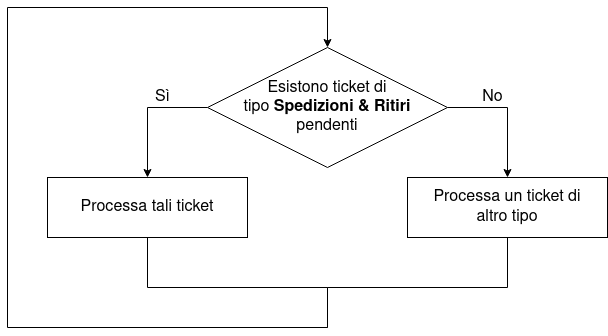
\includegraphics[width=0.75\linewidth]{presentazione-1}
\caption{Schema del comportamento del servente dedicato ai ticket di tipo \sr}
\label{fig:presentazione-1}
\end{figure}

\chapter{Obiettivi dello studio}\label{chp:obiettivi}
L'obiettivo dello studio è quello di minimizzare il numero degli sportelli operativi in un'intera giornata lavorativa, al fine di garantire il soddisfacimento di differenti requisiti di qualità per ciascuna tipologia di servizio illustrata nella presentazione del caso di studio (cap. \ref{chp:presentazione}):

\begin{enumerate}[label=QoS-\arabic*), align=left, leftmargin=*]
\item I clienti titolari di un conto \textsl{BancoPosta} devono sperimentare un tempo d'attesa medio non superiore a $5\ min$.
\item I clienti \textbf{non} titolari di un conto \textsl{BancoPosta}, possessori di ticket di tipo \uo{}, devono sperimentare un tempo d'attesa medio non superiore a $10\ min$.
\item I clienti \textbf{non} titolari di un conto \textsl{BancoPosta}, possessori di ticket di tipo \pp{}, devono sperimentare un tempo d'attesa medio non superiore a $12.5\ min$.
\item I clienti \textbf{non} titolari di un conto \textsl{BancoPosta}, possessori di ticket di tipo \sr{}, devono sperimentare un tempo d'attesa medio non superiore a $15\ min$.
\end{enumerate}
\chapter{Modello concettuale}\label{chp:modello-concettuale}
\begin{figure}[ht]
\centering
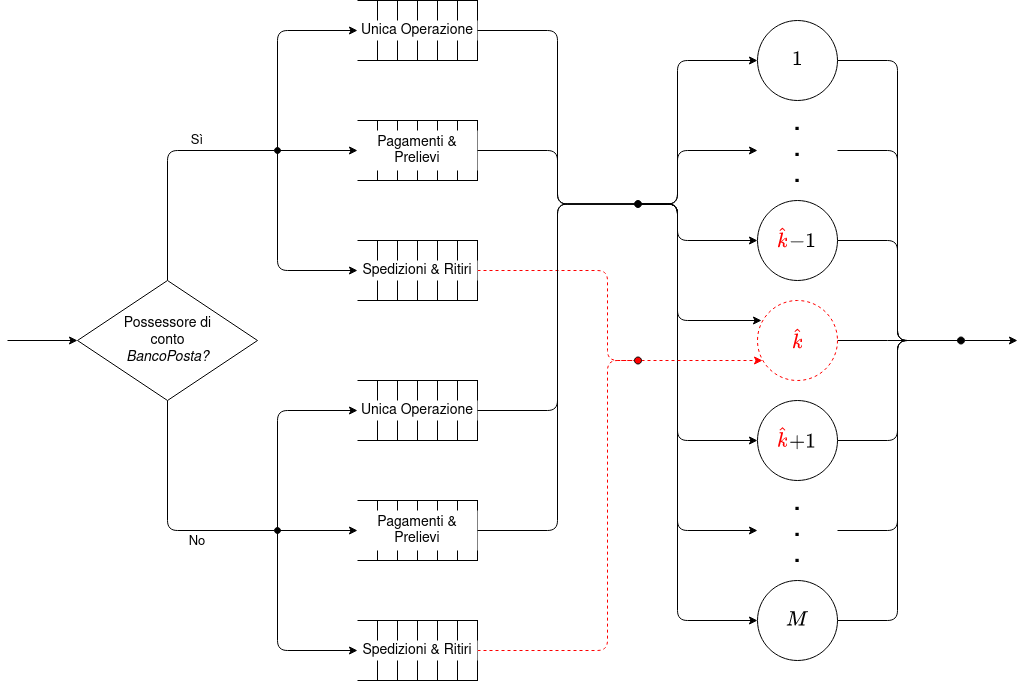
\includegraphics[width=\linewidth]{modello-concettuale-1}
\caption{Diagramma del sistema \textbf{Poste Italiane}}
\label{fig:modello-concettuale-1}
\end{figure}

Il funzionamento del sistema è illustrato dal diagramma in figura \ref{fig:modello-concettuale-1}. Di seguito è riportata una descrizione degli elementi in esso utilizzati:
\begin{itemize}
\item Il rombo rappresenta un meccanismo di ripartizione del flusso in ingresso nelle opportune code, a seconda della titolarità o meno di un conto \textsl{BancoPosta} da parte dei clienti.
\item Ciascuna coda modella una fila di clienti possessori dello stesso tipo di ticket.
\item Ciascun servente rappresenta uno sportello dell'ufficio postale
\begin{itemize}
\item Il $\ded$-esimo servente (evidenziato in {\color{red} rosso}) rappresenta lo sportello dedicato per la gestione dei ticket di tipo \sr{}, il cui comportamento è stato già illustrato nel flow chart in figura \ref{fig:presentazione-1}.
\end{itemize}
\end{itemize}

Ad ogni istante di tempo, lo stato del sistema è univocamente determinato dai valori assunti dalle seguenti $M + 12$ variabili di stato:
\begin{itemize}
\item Per ciascuno degli $M$ sportelli si ha:
\begin{equation}
Server_r \in
\left\lbrace \mathtt{IDLE},\ \mathtt{BUSY} \right\rbrace
\end{equation}
con $r \in \lbrace 1, 2, \dots, M \rbrace$.
\item Per ciascuna delle 6 classi di utenza:
\begin{itemize}
\item Il numero totale di clienti della $c-$esima è modellato dalla variabile $Customers_{c}$
\item Il numero di clienti in servizio della $c-$esima è modellato dalla variabile $InService_{c}$
\end{itemize}
con $c$ appartenente a:
\begin{multicols}{2}
\begin{itemize}
\item \uo{} \textsl{BancoPosta}
\item \pp{} \textsl{BancoPosta}
\item \sr{} \textsl{BancoPosta}
\item \uo{} \textsl{Standard}
\item \pp{} \textsl{Standard}
\item \sr{} \textsl{Standard}
\end{itemize}
\end{multicols}
\end{itemize}

Infine, si assume che:
\begin{itemize}
\item I clienti abbiano un comportamento di tipo \textsl{one-step}\footnote{Avere un comportamento di tipo \textsl{one-step} significa che vi può essere, ad ogni istante di tempo, lo spostamento di un solo cliente alla volta.}.
\item Non è possibile avere uno sportello libero se in coda è presente almeno un cliente con ticket processabile da tale sportello (sistema \textsl{work conserving}\footnote{La proprietà di \textsl{work conserving} è valida entro i vincoli imposti dal caso di studio.}).
\item All'inizio ed alla fine del periodo d'osservazione lo stato del sistema è il seguente:
\begin{equation}
\begin{cases}
Server_r =\mathtt{IDLE} & \forall\ r \\[1em]
Customers_{c} = \mathtt{NONE} & \forall\ c \\[1em]
InService_{c} = \mathtt{NONE} & \forall\ c
\end{cases}
\end{equation}
\end{itemize}
\chapter{Modello delle Specifiche}\label{chp:modello-specifiche}
Le seguenti variabili matematiche, definite per ogni istante di tempo $t$, identificano univocamente una rappresentazione a livello delle specifiche dello stato del sistema:

\begin{itemize}
\item Lo stato dello sportello $r$-esimo è dato da:
\begin{equation}
\label{eqn:modello-specifiche-3}
Server_r(t) \in \lbrace 0, 1 \rbrace
\end{equation}
\item Per ciascuna classe $c$ il numero totale di clienti è definito come:
\begin{equation}
\label{eqn:modello-specifiche-2}
Customers_c(t) \in \mathbb{N}
\end{equation}
\item Per ciascuna classe $c$ il numero di clienti in servizio è definito come segue:
\begin{itemize}
\item Per $c$ diversa da \sr{} \textsl{BancoPosta} e \sr{} \textsl{Standard}:
\begin{equation}
\label{eqn:modello-specifiche-2}
InService_c(t) \in \lbrace 0, 1, \dots, M \rbrace
\end{equation}
\item Altrimenti:
\begin{equation}
\label{eqn:modello-specifiche-2}
InService_c(t) \in \lbrace 0, 1 \rbrace
\end{equation}
\end{itemize}
\end{itemize}

Dalle variabili appena descritte, è immediato ricavare il numero di clienti in coda per ciascuna classe di utenza $c$:
\begin{equation}
Queue_c(t) = Customers_c(t) - InService_c(t)
\end{equation}

Di seguito sono riportate alcune assunzioni che saranno alla base di questa e delle successive fasi dello studio:
\begin{itemize}
\item I clienti arrivano all'ufficio postale ad istanti di tempo casuali, il che implica:
\begin{itemize}
\item Distribuzione poissoniana degli arrivi.
\item Distribuzione esponenziale dei tempi di interarrivo.
\end{itemize}
\item La probabilità che un cliente sia titolare di un conto \textsl{BancoPosta} è pari a $p_{BP} = 0.25$.
\item Le probabilità con cui ciascuna tipologia di ticket viene acquisita sono le seguenti:
\begin{equation*}
\begin{array}{l c l}
\uo{} & \rightarrow & p_{UO} = 0.5 \\
\pp{} & \rightarrow & p_{PP} = 0.35 \\
\sr{} & \rightarrow & p_{SR} = 0.15
\end{array}
\end{equation*} 
\item I tempi di servizio sono distribuiti esponenzialmente.
\item I clienti afferenti ad una stessa coda vengono serviti in accordo ad una disciplina FIFO (First-In, First-Out).
\item Il servizio di un cliente non può essere interrotto per favorire l'avanzamento di un altro con priorità superiore.
\end{itemize}

Al fine di agevolare la comprensione del funzionamento dello scheduler di sistema, di seguito sono riportati gli pseudocodici \ref{alg:modello-specifiche-1} e \ref{alg:modello-specifiche-2} che descrivono, rispettivamente, il comportamento del servente generico e di quello dedicato.

\begin{algorithm}[ht]
\SetAlgoLined
\While{true}{
	\uIf{`\uo{} \textsl{BancoPosta}' queue not empty}{
		\textit{processes the first ticket of that type}\;
	}
	\uElseIf{`\pp{} \textsl{BancoPosta}' queue not empty}{
		\textit{processes the first ticket of that type}\;
	}
	\uElseIf{`\uo{} \textsl{Standard}' queue not empty}{
		\textit{processes the first ticket of that type}\;
	}
	\uElseIf{`\pp{} \textsl{Standard}' queue not empty}{
		\textit{processes the first ticket of that type}\;
	}
	\uElse{
		\textit{do nothing}\;
	}
}
\caption{Algoritmo di schedulazione del servente generico}
\label{alg:modello-specifiche-1}
\end{algorithm}

\begin{algorithm}
\SetAlgoLined
\While{true}{
	\uIf{`\sr{} \textsl{BancoPosta}' queue not empty}{
		\textit{processes the first ticket of that type}\;
	}
	\uElseIf{`\sr{} \textsl{Standard}' queue not empty}{
		\textit{processes the first ticket of that type}\;
	}
	\uElseIf{`\uo{} \textsl{BancoPosta}' queue not empty}{
		\textit{processes the first ticket of that type}\;
	}
	\uElseIf{`\pp{} \textsl{BancoPosta}' queue not empty}{
		\textit{processes the first ticket of that type}\;
	}
	\uElseIf{`\uo{} \textsl{Standard}' queue not empty}{
		\textit{processes the first ticket of that type}\;
	}
	\uElseIf{`\pp{} \textsl{Standard}' queue not empty}{
		\textit{processes the first ticket of that type}\;
	}
	\uElse{
		\textit{do nothing}\;
	}
}
\caption{Algoritmo di schedulazione del servente dedicato}
\label{alg:modello-specifiche-2}
\end{algorithm}

\newpage
In tabella \ref{table:modello-specifiche-1} sono riportati tempi di servizio medi assunti per ciascuna tipologia di ticket, sperimentati su un singolo servente.
\begin{table}[ht]
\centering
{\tablecolors
\begin{tabular}{| l | r |}
\hline
Tipologia di ticket & Tempo di servizio medio \\
\hline
\uo{} & 7 min \\
\hline
\pp{} & 14 min \\
\hline
\sr{} & 10 min \\
\hline
\end{tabular}}
\caption{Assunzioni sui tempi medi di servizio sul singolo sportello}
\label{table:modello-specifiche-1}
\end{table}	

\begin{table}[ht]
\centering
{\tablecolors
\begin{tabular}{| l | r |}
\hline
Grandezza & Valore misurato nel 2018 \\
\hline
N$^o$ di clienti al giorno & 1.5 mln \\
\hline
N$^o$ di uffici postali & 12 812 \\
\hline
\end{tabular}}
\caption{Estratto dei dati di interesse a partire dalla fonte citata}
\label{table:modello-specifiche-2}
\end{table}

Per stimare il throughput dell'intero sistema si è fatto uso dei dati dati provenienti da \textsl{"Principali dati economici e finanziari di Poste Italiane"}\footnote{\url{https://www.posteitaliane.it/it/performance-finanziaria.html}} nel modo seguente:
\begin{equation}
X = \frac{\# \text{clienti al giorno}}{\#\text{uffici postali}} = \frac{1500000}{12812}\ req/wd = \frac{1500000}{12812\cdot 480} \simeq 0.243912\ req/min
\end{equation} 
dove la conversione da giornata lavorativa (\textsl{wd}) a minuti effettivi di lavoro è stata realizzata dividendo per il solo periodo d'erogazione dei ticket. Il motivo è che quest'ultimo ha un'ampiezza fissa, mentre quella del tempo di smaltimento è funzione delle richieste pendenti (cap. \ref{chp:presentazione}). In definitiva, poiché si divide per un numero più piccolo, si effettua una stima per eccesso.

È opportuno osservare che, sotto l'ipotesi di \textsl{job flow balance}, la frequenza d'arrivo media al centro $\lambda$ coincide con il throughput $X$.


\chapter{Modello Computazionale}\label{chp:modello-computazionale}
L'approccio utilizzato per la realizzazione del modello computazionale è quello della next-event simulation. Di seguito è riportata un'analisi delle sue fasi.
\section{Stato del sistema}\label{sec:modello-computazionale-stato}
Le variabili di programma utilizzate per descrivere univocamente lo stato del sistema ad ogni istante di tempo sono:
\begin{itemize}
\item \texttt{{\color{code_purple} int} customers[NUMBER\_OF\_QUEUES]}: vettore di sei interi per la memorizzazione del numero di clienti per ciascuna tipologia di arrivo.
\item \texttt{{\color{code_purple} int} gen\_status[M-1]}: vettore di $M-1$ interi, che assumono valori in accordo alla definizione \ref{eqn:modello-specifiche-3}, per la memorizzazione dello stato dei serventi generali.
\item \texttt{{\color{code_purple} int} ded\_status}: valore intero, che assume valori in accordo alla definizione \ref{eqn:modello-specifiche-4}, per la memorizzazione dello stato del servente dedicato.
\end{itemize}

Il mapping fra le variabili matematiche definite nel modello delle specifiche e quelle di programma a livello computazionale è riassunto nella tabella \ref{table:modello-computazionale-1}. 

\begin{table}[ht]
\centering
{\tablecolors
\begin{tabular}{| l | l |}
\hline
Variabile matematica & Variabile di programma \\
\hline
$Customers_i(t)$ & \texttt{{\color{code_purple}int} customers[i]} \\
\hline
$Server_r(t)$ & \texttt{{\color{code_purple}int} gen\_status[r]} \\
\hline
$Server_\ded(t)$ & \texttt{{\color{code_purple}int} ded\_status} \\
\hline
\end{tabular}}
\caption{Mapping tra il modello delle specifiche e quello computazionale}
\label{table:modello-computazionale-1}
\end{table}
\newpage
Ad inizio simulazione lo stato del sistema viene impostato come mostrato nello snippet \ref{lst:modello-computazionale-1}.
\lstinputlisting[label={lst:modello-computazionale-1}, caption={Inizializzazione dello stato del sistema}, firstline=69, lastline=72]{../src/simul.c}
\section{Eventi}\label{sec:modello-computazionale-eventi}
Siano:
\begin{itemize}
\item \texttt{i} l'indice che assume valori appartenenti alla terza colonna della tabella \ref{table:modello-specifiche-1} ($\mathtt{i} \neq -1$).
\item \texttt{r} l'indice che assume valori appartenenti all'insieme $\mathtt{\lbrace 0, 1, \dots, M - 2 \rbrace}$, utilizzato per accedere ai record dell'array \texttt{gen\_status}.
\end{itemize}
Lo stato del sistema può cambiare all'occorrenza delle seguenti tipologie di eventi propri:
\begin{itemize}
\item Sei tipologie d'arrivi, all'occorrenza dei quali:
\begin{center}
\texttt{customers[i] = customers[i] + 1}
\end{center}
\item Due tipologie di completamenti per ciascun server generale, a seguito dei quali:
\begin{itemize}
\item \texttt{gen\_status[r]} passa da un certo valore \texttt{i} ad \texttt{IDLE}
\item \texttt{customers[i] = customers[i] - 1}
\end{itemize}
\item Tre tipologie di completamenti per il server dedicato che comportano:
\begin{itemize}
\item \texttt{ded\_status} passa da un certo valore \texttt{i} ad \texttt{IDLE}
\item \texttt{customers[i] = customers[i] - 1}
\end{itemize}
\end{itemize} 
\section{Clock di simulazione}\label{sec:modello-computazionale-clock}
L'orologio di sistema adottato nel simulatore è contenuto all'interno di una struttura dati\footnote{Nel codice viene adottata la variabile globale \texttt{{\color{code_purple}times\_t} t}.}, riportata nello snippet \ref{lst:modello-computazionale-2}, che memorizza informazioni relative al tempo di simulazione. In particolare:
\begin{itemize}
\item \texttt{{\color{code_purple}double} next}: istante di occorenza del successivo evento nel sistema.
\item \texttt{{\color{code_purple}double} last[NUMBER\_OF\_QUEUES]}: ciascuna entry \texttt{i} rappresenta l'istante dell'ultimo arrivo di tipo \texttt{i}.
\item \texttt{{\color{code_purple}double} current}: orologio di sistema.
\end{itemize}

\lstinputlisting[label={lst:modello-computazionale-2}, caption={Struttura dati per la gestione del tempo}, firstline=60, lastline=64]{../src/simul.c}
Di seguito sono riportate alcune osservazioni relative al tempo di simulazione:
\begin{itemize}
\item L'unità di misura di riferimento è il minuto.
\item L'orologio di sistema (\texttt{t->current}) viene inizializzato a \texttt{START}.
\item Il tempo di simulazione $\tau$ è pari a \texttt{STOP}.
\item Nel caso in cui un'istante di arrivo $t^*$ sia postumo al termine della simulazione ($t^* > \tau$), il suo tempo di occorrenza viene impostato pari a \texttt{INFTY} per denotare il blocco di quel flusso di arrivi (\textit{"close the door"}).
\end{itemize}
Per il caso di studio in analisi è stata adottata la seguente configurazione di parametri:
\begin{center}
\begin{tabular}{l c r}
\texttt{START = 0}, & \texttt{STOP = 480\footnotemark}, & \texttt{INFTY = 100 $\cdot$ STOP}
\end{tabular}
\footnotetext{Numero medio di minuti di una giornata lavorativa, calcolato a partire dalla \ref{eqn:modello-specifiche-15}.}
\end{center}
\section{Scheduler}\label{sec:modello-computazionale-scheduler}
Il meccanismo di avanzamento del tempo, che garantisce l'occorrenza ordinata degli eventi temporali, ad ogni iterazione del loop di simulazione:
\begin{enumerate}
\item Computa l'occorrenza del next-event (\texttt{t->next = next\_event(\dots)})
\item Aggiorna l'orologio di sistema (\texttt{t->current = t->next})
\end{enumerate}
fintantoché è verificata almeno una delle seguenti due condizioni:
\begin{itemize}
\item Il tempo di occorrenza degli eventi è non superiore a $\tau$.
\item Sono presenti clienti nel sistema non ancora serviti.
\end{itemize}

\section{Lista degli eventi}\label{sec:modello-computazionale-lista-eventi}
La lista degli eventi, a livello implementativo, è gestita mediante la struttura dati\footnote{Nel codice viene adottata la variabile globale \texttt{{\color{code_purple}event\_list\_t} events}.} riportata nello snippet \ref{lst:modello-computazionale-3}.
Ciascun campo della struttura mantiene gli istanti di tempo di occorrenza di una categoria di eventi. In particolare:
\begin{itemize}
\item \texttt{{\color{code_purple}double} arrivals[NUMBER\_OF\_QUEUES]}: ciascuna entry \texttt{i} rappresenta l'istante del successivo arrivo di tipo \texttt{i}.
\item \texttt{{\color{code_purple}double} gen\_completions[M-1]}: ciascuna entry \texttt{r} rappresenta l'istante del successivo completamento del server \texttt{r}.
\item \texttt{{\color{code_purple}double} ded\_completion}: rappresenta l'istante del successivo completamento del server dedicato.
\end{itemize}

\lstinputlisting[label={lst:modello-computazionale-3}, caption={Struttura dati per la lista degli eventi}, firstline=54, lastline=58]{../src/simul.c}
\section{Algoritmo next-event}\label{sec:modello-computazionale-algoritmo}
L'algoritmo di simulazione implementato consiste nei seguenti quattro passi:
\begin{enumerate}[label=Step \arabic*), align=left, leftmargin=*]
\item \textbf{Inizializzazione}
\begin{itemize}
\item L'orologio di simulazione è inizializzato come descritto nella sezione \ref{sec:modello-computazionale-clock}.
\item La lista degli eventi (\texttt{events}) è inizializzata determinando la prima occorrenza di ogni possibile evento. In particolare:
\begin{center}
\begin{tabular}{l l l}
\texttt{events->arrivals[i]} & \texttt{=} & \texttt{GetArrival(i)} \\
\texttt{events->gen\_completions[i]} & \texttt{=} & \texttt{INFTY} \\
\texttt{events->ded\_completion} & \texttt{=} & \texttt{INFTY}
\end{tabular}
\end{center}
\end{itemize}
\item \textbf{Processamento evento corrente}
\begin{enumerate}
\item La lista degli eventi è scandita per determinare l'evento più imminente possibile, in accordo a quanto descritto nella sezione \ref{sec:modello-computazionale-scheduler}.
\item L'orologio di sistema viene avanzato al tempo di occorrenza dell'evento schedulato, in relazione a quanto proposto in sezione \ref{sec:modello-computazionale-scheduler}.
\item L'evento schedulato viene processato, come illustrato in sezione \ref{sec:modello-computazionale-eventi}.
\end{enumerate}
\item \textbf{Schedulazione nuovi eventi}
\begin{itemize}
\item Nel caso in cui l'evento corrente sia un arrivo di tipo $\mathtt{i \in \lbrace 0, 1, 2, 3 \rbrace}$:
\begin{itemize}
\item Se esiste almeno un servente generale \texttt{r} che è \texttt{IDLE}:
\begin{center}
\begin{tabular}{l l l}
\texttt{gen\_status[r]} & \texttt{=} & \texttt{i} \\
\texttt{events->gen\_completions[r]} & \texttt{=} & \texttt{t->current + GetService(i)}
\end{tabular}
\end{center}
\item Altrimenti, se il servente dedicato è \texttt{IDLE}:
\begin{center}
\begin{tabular}{l l l}
\texttt{ded\_status} & \texttt{=} & \texttt{i} \\
\texttt{ded\_completion} & \texttt{=} & \texttt{t->current + GetService(i)}
\end{tabular}
\end{center}
\end{itemize}
\item Nel caso in cui l'evento corrente sia un arrivo di tipo $\mathtt{i \in \lbrace 4, 5 \rbrace}$, se il servente dedicato è \texttt{IDLE}:
\begin{center}
\begin{tabular}{l l l}
\texttt{ded\_status} & \texttt{=} & \texttt{i} \\
\texttt{ded\_completion} & \texttt{=} & \texttt{t->current + GetService(i)}
\end{tabular}
\end{center}
\item Nel caso in cui l'evento corrente sia un completamento di tipo $\mathtt{i \in \lbrace 0, 1, 2, 3 \rbrace}$ da parte di un server generale \texttt{r}:
\begin{center}
\texttt{customers[i] = customers[i] - 1}
\end{center}
\begin{itemize}
\item Se esiste almeno una richiesta di tipo $\mathtt{j \in \lbrace 0, 1, 2, 3 \rbrace}$ in attesa di essere servita\footnote{\label{note:modello-computazionale-1}Nel caso in cui vi fossero più code non vuote, la priorità verrebbe data a quella con indice \texttt{j} minore.}:
\begin{center}
\begin{tabular}{l l l}
\texttt{gen\_status[r]} & \texttt{=} & \texttt{j} \\
\texttt{events->gen\_completions[r]} & \texttt{=} & \texttt{t->current + GetService(j)}
\end{tabular}
\end{center}
\item Altrimenti:
\begin{center}
\begin{tabular}{l l l}
\texttt{gen\_status[r]} & \texttt{=} & \texttt{IDLE} \\
\texttt{events->gen\_completions[r]} & \texttt{=} & \texttt{INFTY}
\end{tabular}
\end{center}
\end{itemize}
\item Nel caso in cui l'evento corrente sia un completamento di tipo $\mathtt{i \in \lbrace 0, \dots, 5 \rbrace}$ da parte del server dedicato:
\begin{center}
\texttt{customers[i] = customers[i] - 1}
\end{center}
\begin{itemize}
\item Se esiste almeno una richiesta di tipo $\mathtt{j \in \lbrace 4, 5 \rbrace}$ in attesa di essere servita\textsuperscript{\ref{note:modello-computazionale-1}}:
\begin{center}
\begin{tabular}{l l l}
\texttt{ded\_status} & \texttt{=} & \texttt{j} \\
\texttt{events->ded\_completion} & \texttt{=} & \texttt{t->current + GetService(j)}
\end{tabular}
\end{center}
\item Altrimenti, se esiste almeno una richiesta di tipo $\mathtt{j \in \lbrace 0, 1, 2, 3 \rbrace}$ in attesa di essere servita\textsuperscript{\ref{note:modello-computazionale-1}}:
\begin{center}
\begin{tabular}{l l l}
\texttt{ded\_status} & \texttt{=} & \texttt{j} \\
\texttt{events->ded\_completion} & \texttt{=} & \texttt{t->current + GetService(j)}
\end{tabular}
\end{center}
\item Altrimenti:
\begin{center}
\begin{tabular}{l l l}
\texttt{ded\_status} & \texttt{=} & \texttt{IDLE} \\
\texttt{events->ded\_completion} & \texttt{=} & \texttt{INFTY}
\end{tabular}
\end{center}
\end{itemize}
\end{itemize}
\item \textbf{Terminazione}
\begin{itemize}
\item L'evento artificiale che causa la terminazione della simulazione è l'intersezione dei seguenti:
\begin{itemize}
\item La prossima occorrenza di una qualsiasi tipologia di arrivo è postuma a $\tau$ (\texttt{events->arrivals[i] > STOP} per ogni \texttt{i}).
\item Non sono presenti richieste da processare (\texttt{customers[i] = 0} per ogni \texttt{i}).
\end{itemize}
\end{itemize}
\end{enumerate}
\chapter{Verifica}\label{chp:verifica}
In fase di verifica si è fatto uso della funzione \texttt{print\_update(\dots)} per monitorare l'avanzamento della simulazione \textit{step-by-step}, con l'obiettivo di controllare che l'evoluzione dello stato del sistema avvenisse fedelmente ai modelli precedentemente descritti (capp. \ref{chp:modello-concettuale}, \ref{chp:modello-specifiche}, \ref{chp:modello-computazionale}).

\begin{figure}[ht]
\centering
\begin{subfigure}[b]{0.475\textwidth}
\centering
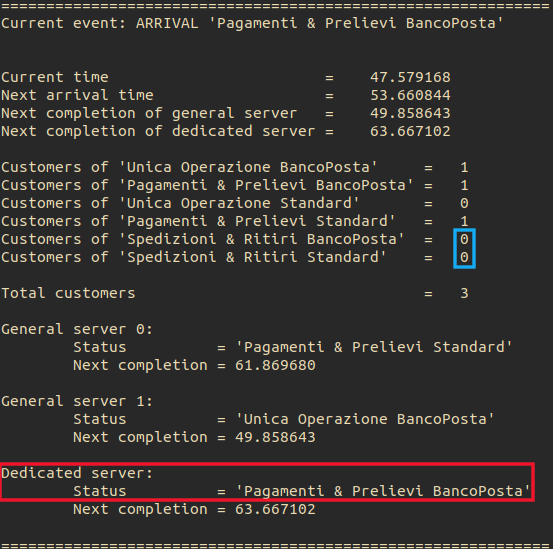
\includegraphics[width=\textwidth]{screenshots/original/ded_server_changes_behaviour}
\caption{Cambio del comportamento del server dedicato}    
\label{fig:verifica-1a}
\end{subfigure}
\hfill    
\begin{subfigure}[b]{0.475\textwidth}  
\centering 
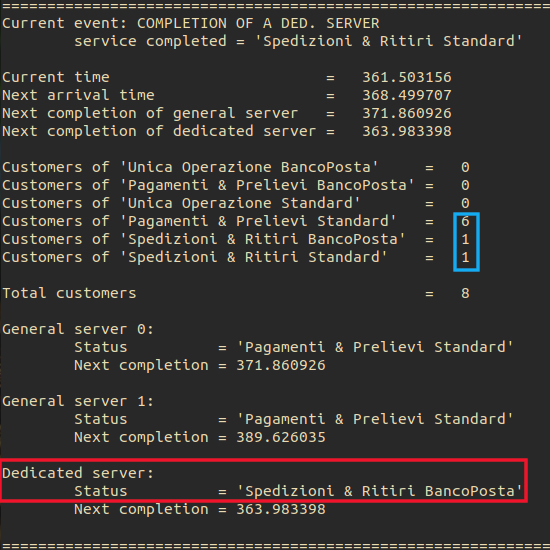
\includegraphics[width=\textwidth]{screenshots/original/ded_server_priority_sched}
\caption{Schedulazione sul server dedicato}    
\label{fig:verifica-1b}
\end{subfigure}


\vskip\baselineskip

\begin{subfigure}[b]{0.475\textwidth}   
\centering 
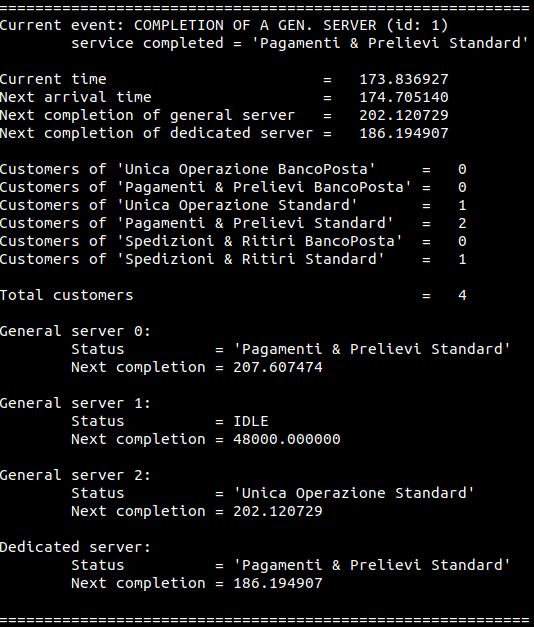
\includegraphics[width=\textwidth]{screenshots/original/gen_servers_no_SR}
\caption{I server generali non processano \sr{}}   
\label{fig:verifica-1c}
\end{subfigure}
\hfill
\begin{subfigure}[b]{0.475\textwidth}   
\centering 
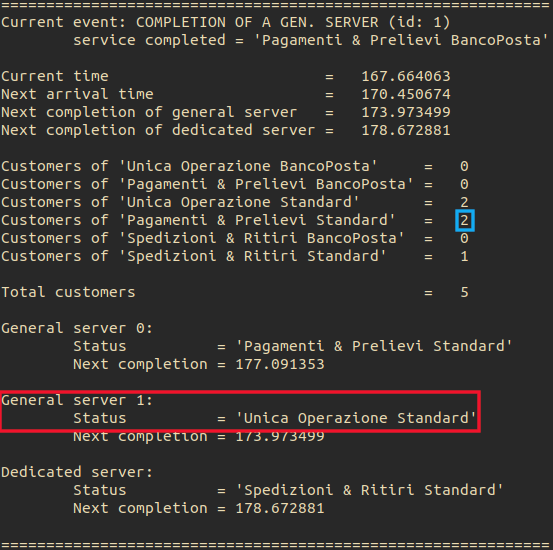
\includegraphics[width=\textwidth]{screenshots/original/gen_servers_priority_sched}
\caption{Schedulazione su un server generale}    
\label{fig:verifica-1d}
\end{subfigure}
\caption{Screenshots della simulazione per la fase di verifica}
\label{fig:verifica-1}
\end{figure}

I controlli di consistenza effettuati sono di seguito analizzati:
\begin{itemize}
\item In assenza di ticket di tipo \sr{} da processare, il server dedicato si comporta come se fosse generale, ovvero elaborando, se presenti, richieste \uo{} o \pp{} (fig. \ref{fig:verifica-1a}).
\item In presenza di ticket di tipo \sr{} da processare, il server dedicato ignora le altre code e processa tali richieste dando priorità ai titolari di conto \textsl{BancoPosta} (fig. \ref{fig:verifica-1b}).
\item Pur essendo \texttt{IDLE}, i server generali non possono processare richieste di tipo \sr{} (fig. \ref{fig:verifica-1c}).
\item Un server è \texttt{IDLE} se e solo se non sono presenti richieste pendenti che è in grado di processare (fig. \ref{fig:verifica-1c}).
\item In fase di schedulazione, i server generali processano le richieste secondo l'ordine di priorità specificato nei modelli precedenti (fig. \ref{fig:verifica-1d}).
\end{itemize}

In particolare, gli screenshot riportati in figura \ref{fig:verifica-1}, e sopra più volte referenziati, sono stati tutti quanti realizzati fissando come seed iniziale \texttt{9}.
\chapter{Validazione}\label{chp:validazione}
Poiché i risultati dei modelli analitici sono validi per periodi d'osservazione tendenzialmente infiniti, è stato scelto in fase di validazione di adottare una simulazione di tipo \textit{steady-state}, al fine di inferire statistiche confrontabili con i valori teorici.

Il metodo adottato è stato quello delle batch means con parametri $(b,k) = (256, 64)$ e periodo d'osservazione $\tau = 16384\ min$. La scelta dei parametri è stata effettuata seguendo le linee guida\footnote{Capitolo 8 del libro \textit{"Discrete Event Simulation - A First Course - Lemmis Park"}.}:
\begin{itemize}
\item $b = 256$, rappresenta un buon compromesso fra il mantenimento della variabilità naturale del fenomeno osservato e l'indipendenza tra batch successivi.
\item $k = 64$, al fine di rendere le statistiche campionate indipendenti dalle
condizioni iniziali ed ottenere intervalli di confidenza significativi.
\end{itemize}

Inoltre:
\begin{itemize}
\item Il seed iniziale utilizzato per le simulazioni che seguono in questo capitolo è \texttt{12345}.
\item È stato utilizzato il programma \texttt{estimate} per il calcolo delle realizzazioni degli intervalli di confidenza.
\end{itemize}

\section{Definizione preliminare dei modelli analitici semplificati}
\begin{figure}[ht]
\centering
\begin{subfigure}[b]{0.475\textwidth}  
\centering 
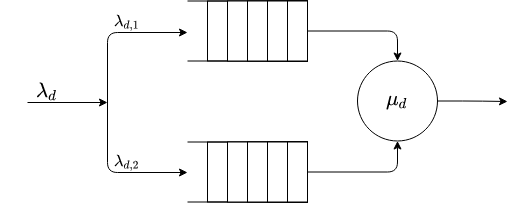
\includegraphics[width=\textwidth]{validazione-modello-analitico-1a}
\caption{Blocco dei ticket \sr{}}    
\label{fig:validazione-modello-analitico-1a}
\end{subfigure}
\hfill 
\begin{subfigure}[b]{0.475\textwidth}
\centering
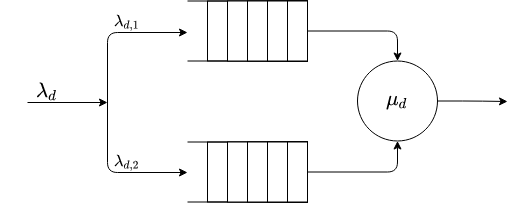
\includegraphics[width=\textwidth]{validazione-modello-analitico-1b}
\caption{Blocco delle altre tipologie di ticket}    
\label{fig:validazione-modello-analitico-1b}
\end{subfigure}
\caption{Modelli analitici semplificati}
\label{fig:validazione-modello-analitico-1}
\end{figure}

Di seguito è riportata un'analisi teorica della rete di Jackson in figura \ref{fig:validazione-modello-analitico-1} necessaria alle sezioni successive della validazione.


\subsection{Descrizione del modello in figura \ref{fig:validazione-modello-analitico-1a}}
Al fine di rendere i risultati teorici confrontabili con quelli della simulazione, si assume che nel modello in figura \ref{fig:validazione-modello-analitico-1a} il servente abbia capacità $M$ volte superiore a quella dei singoli serventi nel multiserver del modello di riferimento.

I parametri di input del sistema \ref{fig:validazione-modello-analitico-1a} sono di seguito riportati:
\begin{itemize}
\item Le probabilità di ricadere in una determinata classe di priorità, sono pari a:
\begin{equation}
\begin{array}{l l}
p_{g,1} = \frac{p_{BP} \cdot p_{UO}}{p_{UO} + p_{PP}} = 0.147059, & p_{g,2} = \frac{p_{BP} \cdot p_{PP}}{p_{UO} + p_{PP}} = 0.102941, \\[1em]
p_{g,3} = \frac{(1-p_{BP}) \cdot p_{UO}}{p_{UO} + p_{PP}} = 0.441176, & p_{g,4} = \frac{(1-p_{BP}) \cdot p_{PP}}{p_{UO} + p_{PP}} = 0.308824, \\[1.5em]
\end{array}
\end{equation}
dove il fattore $\frac{1}{p_{UO} + p_{PP}}$ è necessario per normalizzare le probabilità originali.

\item Definito:
\begin{equation}
\lambda_g = (p_{UO} + p_{PP})\cdot \lambda = 0.207325\ req/min
\end{equation} 

I tassi medi d'arrivo sono pari a:
\begin{equation}
\begin{array}{l l}
\lambda_{g,1} = p_{g,1} \cdot \lambda_g \simeq 0.030489\ req/min, & \lambda_{g,2} = p_{g,2} \cdot \lambda_g \simeq 0.021342\ req/min, \\
\lambda_{g,3} = p_{g,3} \cdot \lambda_g \simeq 0.091467\ req/min, & \lambda_{g,4} = p_{g,4} \cdot \lambda_g \simeq 0.064027\ req/min, \\[1em]
\end{array}
\end{equation}

\item Il tasso di servizio medio è pari a:
\begin{equation}
\label{eqn:validazione-6}
\mu_g = \frac{1}{E[S_g]} = \frac{M}{\frac{14+7}{2}} = \frac{2M}{21}\ req/min
\end{equation}
dove per il calcolo di $E[S_g]$ è stata utilizzata la media dei tempi di servizio delle richieste relative ai ticket \uo{} e \pp{}, assunti in tabella \ref{table:modello-specifiche-1} nel modello delle specifiche.

\item L'occupazione media delle classi $\rho_{g,i} = \lambda_{g,i}/\mu_g$ è pari a:
\begin{equation}
\begin{array}{l l l l}
\rho_{g,1} = \frac{0.320135}{M}, & \rho_{g,2} = \frac{0.224091}{M}, & \rho_{g,3} = \frac{0.960404}{M}, & \rho_{g,4} = \frac{0.672284}{M} \\[1.5em]
\end{array}
\end{equation}
da cui:
\begin{equation}
\label{eqn:validazione-8}
\rho_g = \sum_{i=1}^4 \rho_{g,i} = \frac{2.176914}{M}
\end{equation}
Dalla \ref{eqn:validazione-8} è immediato osservare che è necessario imporre $M \geq 3$ al fine di garantire la stabilità del sistema.
\end{itemize}

Tale sistema è modellato con una coda $M/M/1$ in cui si adotta una disciplina di scheduling astratta. A tal proposito, è possibile utilizzare la KP per calcolare gli indici globali necessari alla validazione, come segue:
\begin{itemize}
\item Il \textbf{tempo medio d'attesa} globale è pari a:
\begin{equation}
\label{eqn:validazione-11}
E[T_{Q_g}]^{KP} = \frac{\rho_g E[S_g]}{1-\rho_g} = \frac{22.8576}{M\cdot (M-2.17691)}\ min
\end{equation}
\item Il \textbf{tempo medio di risposta} globale è pari a:
\begin{equation}
\label{eqn:validazione-13}
E[T_{S_g}] = \frac{1}{\mu_g - \lambda_g} = \frac{10.5}{M-2.17691}\ min
\end{equation}
\end{itemize}

\subsection{Descrizione del modello in figura \ref{fig:validazione-modello-analitico-1b}}

I parametri di input del sistema \ref{fig:validazione-modello-analitico-1b} sono di seguito riportati:
\begin{itemize}
\item Le probabilità di ricadere in una determinata classe di priorità, sono pari a:
\begin{equation}
\begin{array}{l l}
p_{d,1} = \frac{p_{BP} \cdot \cancel{p_{SR}}}{\cancel{p_{SR}}} = 0.25, & p_{d,2} = \frac{(1-p_{BP}) \cdot \cancel{p_{SR}}}{\cancel{p_{SR}}} = 0.75
\end{array}
\end{equation}
dove il fattore $\frac{1}{p_{SR}}$ normalizza le probabilità originali.

\item Definito:
\begin{equation}
\lambda_d = p_{SR}\cdot \lambda = 0.036587\ req/min
\end{equation} 

I tassi medi d'arrivo sono pari a:
\begin{equation}
\begin{array}{l l}
\lambda_{d,1} = p_{d,1} \cdot \lambda_d \simeq 0.009147\ req/min, & \lambda_{d,2} = p_{d,2} \cdot \lambda_d \simeq 0.027440\ req/min
\end{array}
\end{equation}

\item Il tasso di servizio medio è pari a:
\begin{equation}
\mu_d = \frac{1}{E[S_d]} = \frac{1}{10} = 0.1\ req/min
\end{equation}
in accordo alle assunzioni in tabella \ref{table:modello-specifiche-1} nel modello delle specifiche.

\item L'occupazione media delle classi $\rho_{d,j} = \lambda_{d,j}/\mu_d$ è pari a:
\begin{equation}
\begin{array}{l l}
\rho_{d,1} = 0.09147, & \rho_{d,2} = 0.27440
\end{array}
\end{equation}
da cui:
\begin{equation}
\rho_d = \rho_{d,1} + \rho_{d,2} = 0.36587
\end{equation}
\end{itemize}

Tale sistema è modellato con una coda $M/M/1$ in cui si adotta una disciplina di scheduling astratta. A tal proposito, è possibile utilizzare la KP per calcolare gli indici globali necessari alla validazione, come segue:
\begin{itemize}
\item Il \textbf{tempo medio d'attesa} globale, per il sottosistema in figura \ref{fig:validazione-modello-analitico-1b} è pari a:
\begin{equation}
\label{eqn:validazione-24}
E[T_{Q_d}]^{KP} = \frac{\rho_d \cdot E[S_d]}{1-\rho_d} = 5.769637\ min
\end{equation}
\item Il \textbf{tempo medio di risposta} globale, per il sottosistema in figura \ref{fig:validazione-modello-analitico-1b} è pari a:
\begin{equation}
\label{eqn:validazione-26}
E[T_{S_d}] = \frac{1}{\mu_d - \lambda_d} = 15.769637\ min
\end{equation}
\end{itemize}


\section{Blocco del flusso degli arrivi di tipo \sr{}}\label{sec:validazione-blocco-sr}
\begin{figure}[ht]
\centering
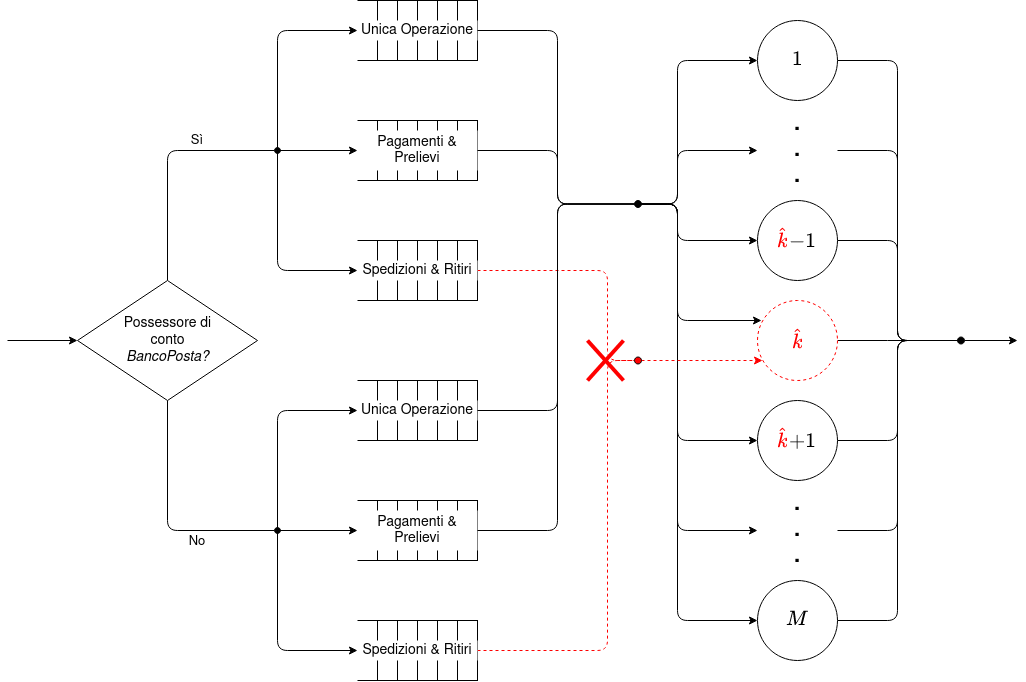
\includegraphics[width=0.5\linewidth]{modello-concettuale-sempl-1}
\caption{Blocco del flusso degli arrivi di tipo \sr{}}
\label{fig:validazione-semplificazione-1}
\end{figure}
Privando il sistema della generazione di arrivi di tipo \sr{}, come mostrato in figura \ref{fig:validazione-semplificazione-1} e fissando $M=3$, si ottengono i seguenti risultati:
\begin{itemize}
\item Mediante la simulazione:
\begin{itemize}
\item Un intervallo di confidenza al 95\% per il tempo medio d'attesa globale è pari a:
\begin{equation} 
\bar{d}_g = \sum_{i = 1}^4 p_{g,i}\cdot \bar{d}_{g,i} = (4.29 \pm 1.02)\ min
\end{equation}
\item Un intervallo di confidenza al 95\% per il tempo medio di risposta globale è pari a:
\begin{equation}
\bar{w}_g = \sum_{i = 1}^4 p_{g,i}\cdot \bar{w}_{g,i} = (14.56 \pm 1.29)\ min
\end{equation}
\end{itemize}

\item Mediante l'analisi effettuata in riferimento al modello a code riportato in figura \ref{fig:validazione-modello-analitico-1a}:
\begin{itemize}
\item Il tempo medio d'attesa globale ottenuto è pari a:
\begin{equation}
E[T_{Q_g}]^{KP} = 9.256825\ min 
\end{equation}
\item Il tempo medio di risposta globale ottenuto è pari a:
\begin{equation}
E[T_{S_g}] = 12.756807\ min 
\end{equation}
\end{itemize}
in accordo rispettivamente alle equazioni \ref{eqn:validazione-11} e \ref{eqn:validazione-13}.
\end{itemize}

I risultati ottenuti sono ragionevoli poiché:
\begin{itemize}
\item Il tempo d'attesa medio di un multiserver, a parità di utilizzazione, è teoricamente inferiore a quello di un single server a capacità equivalente, per via del fatto che $P_Q \leq \rho$.
\item Il tempo di risposta medio di un multiserver è asintoticamente equivalente a quello di un single server avente la medesima capacità nel caso in cui $\rho\to 1$. In questo caso, poiché:
\begin{itemize}
\item Un intervallo di confidenza al 95\% per l'occupazione media ottenuta tramite la simulazione è pari a:
\begin{equation}
\bar{x}_g = 0.70 \pm 0.03
\end{equation}
\item L'occupazione media teorica, in accordo alla \ref{eqn:validazione-8}, è pari a:
\begin{equation}
\rho_g = 0.725638
\end{equation}
\end{itemize}
le prestazioni del multiserver, in termini di risposta, sono inferiori al sistema a capacità concentrata.
\end{itemize}

È opportuno osservare che i risultati ottenuti in fase di simulazione sono stati computati mantenendo i tassi di servizio delle differenti tipologie di ticket, così come definiti nel modello delle specifiche (cap. \ref{chp:modello-specifiche}). Questo è ragionevole perché la media pesata dei differenti tassi di servizio è pari a quello definito nella \ref{eqn:validazione-6}.


\section{Blocco del flusso degli arrivi di tipo \uo{} e \pp{}}\label{sec:validazione-blocco-uo-pp}
Privando il sistema della generazione di arrivi di tipo \uo{} e \pp{}, come mostrato in figura \ref{fig:validazione-semplificazione-2}, si ottengono i seguenti risultati:
\begin{itemize}
\item Mediante la simulazione:
\begin{itemize}
\item Un intervallo di confidenza al 95\% per il tempo medio d'attesa globale ottenuto è pari a:
\begin{equation} 
\bar{d}_d = p_{d,1}\cdot \bar{d}_{d,1} + p_{d,2}\cdot \bar{d}_{d,2} = (6.04 \pm 1.88)\ min
\end{equation}
\item Un intervallo di confidenza al 95\% per il tempo medio di risposta globale ottenuto è pari a:
\begin{equation}
\bar{w}_d = p_{d,1}\cdot \bar{w}_{d,1} + p_{d,2}\cdot \bar{w}_{d,2} = (16.45 \pm 2.64)\ min
\end{equation}
\end{itemize}

\item Mediante l'analisi effettuata in riferimento al modello a code riportato in figura \ref{fig:validazione-modello-analitico-1b}:
\begin{itemize}
\item Il tempo medio d'attesa globale ottenuto è pari a:
\begin{equation}
E[T_{Q_d}]^{KP} = 5.769637\ min 
\end{equation}
\item Il tempo medio di risposta globale ottenuto è pari a:
\begin{equation}
E[T_{S_d}] = 15.769637\ min 
\end{equation}
\end{itemize}
in accordo rispettivamente alle equazioni \ref{eqn:validazione-24} e \ref{eqn:validazione-26}.
\end{itemize}

Poiché i valori teorici ricadono all'interno dei rispettivi intervalli, con un livello di confidenza del 95\%, il comportamento del simulatore è conforme al modello analitico \ref{fig:validazione-modello-analitico-1b}.

\begin{figure}[ht]
\centering
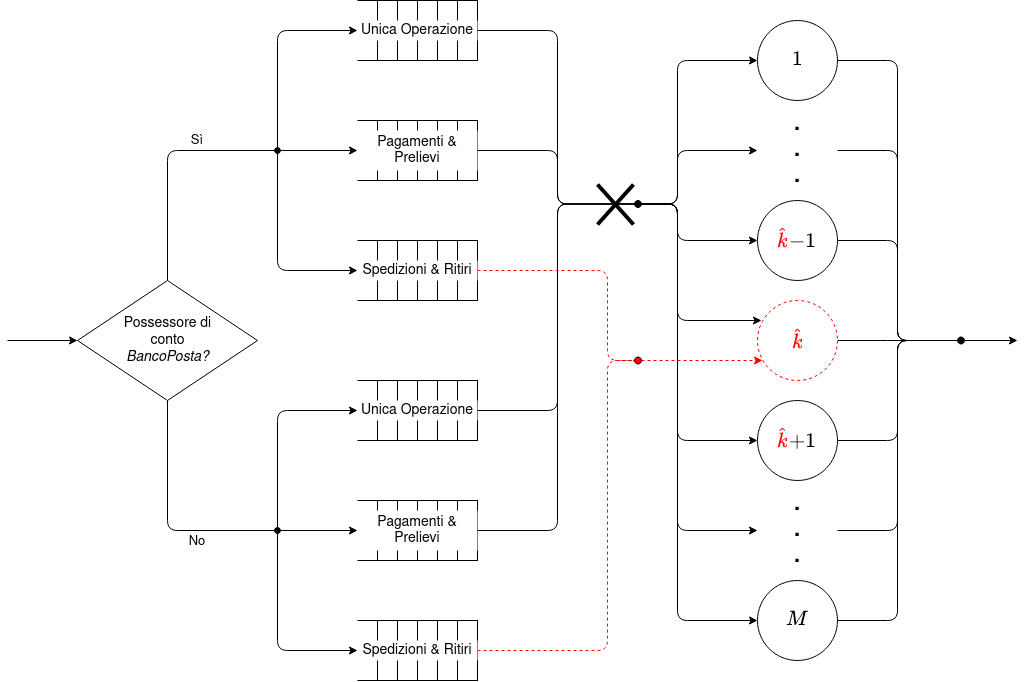
\includegraphics[width=0.5\linewidth]{modello-concettuale-sempl-2}
\caption{Blocco del flusso degli arrivi di tipo \uo{} e \pp{}}
\label{fig:validazione-semplificazione-2}
\end{figure}


\end{document}